\chapter{Обзор алгоритмов управления скоростью}
\label{cha:chap2}

\section{ПИ (ПИД) регулятор}
\label{sec:pid}

В качестве простейшего регулятора скорости может быть использован ПИ или ПИД регулятор по скорости. Схема реализации приведена на Рисунке \ref{pic:pid1}.

\begin{figure}[!h]
\centering
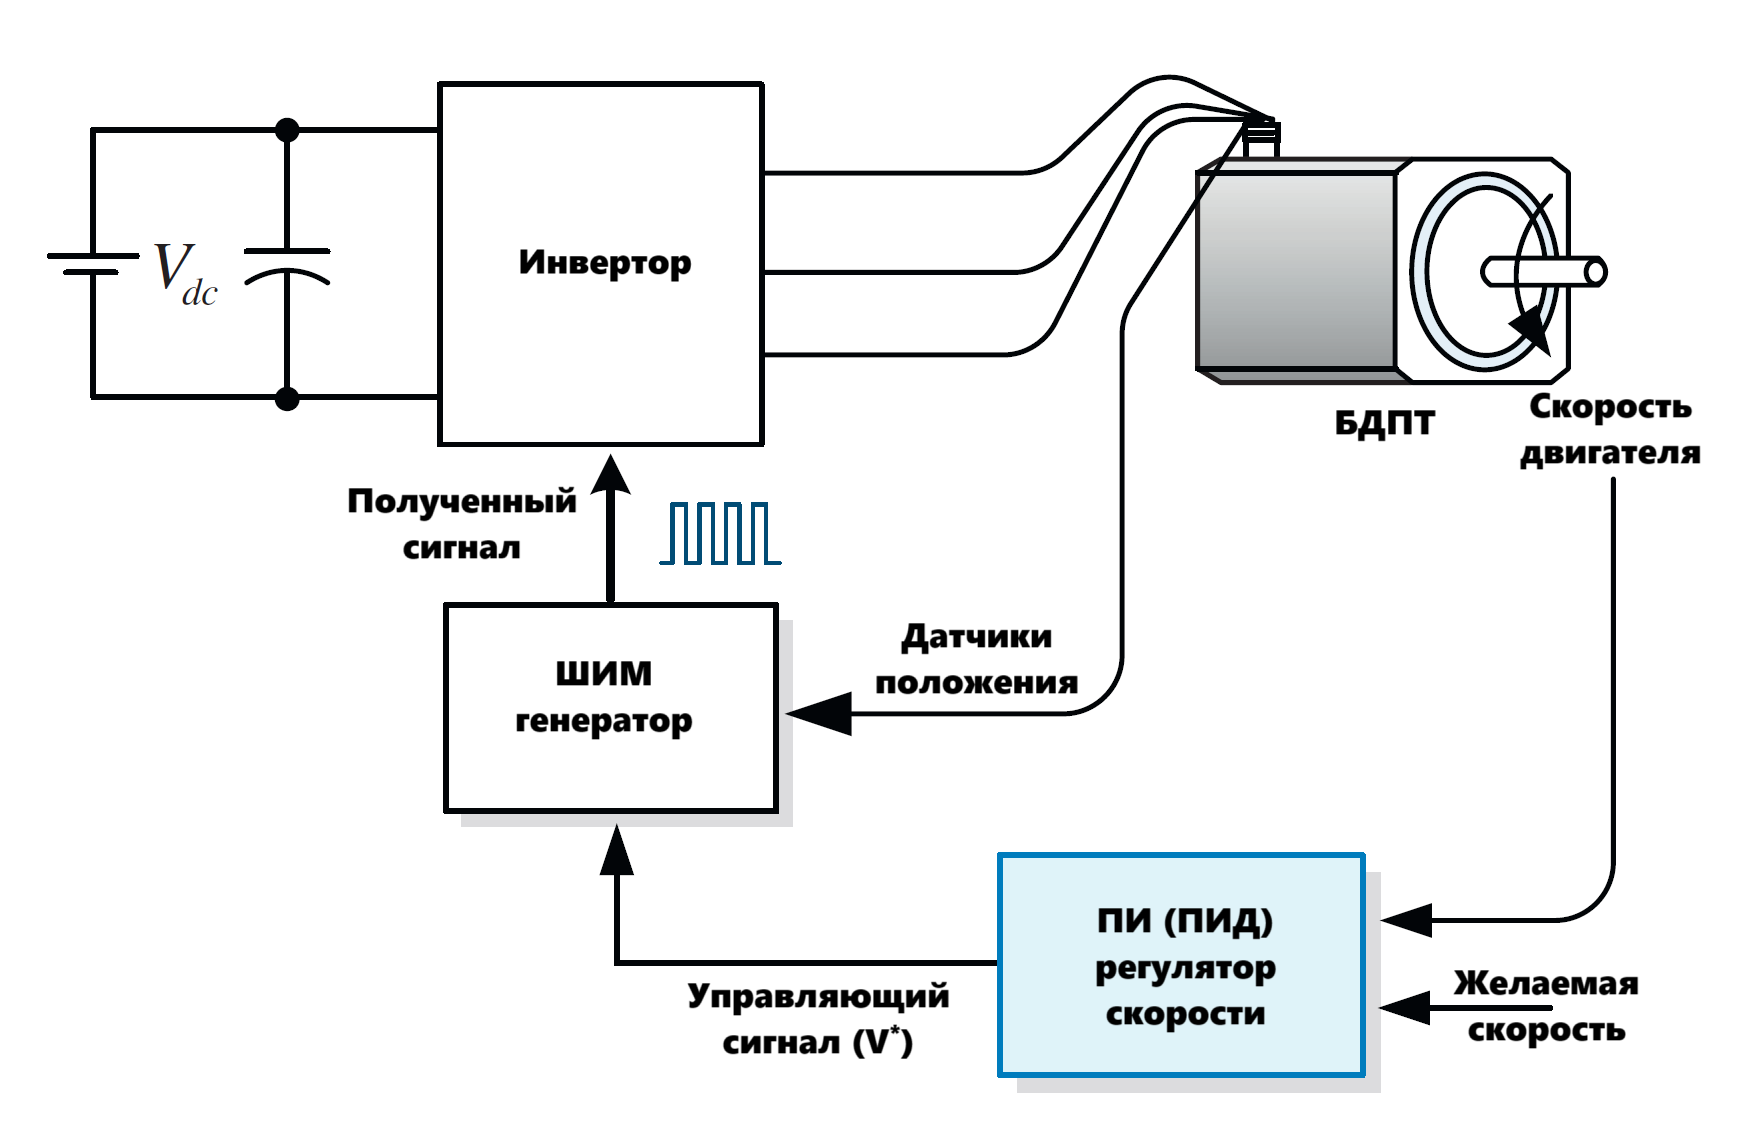
\includegraphics[width=0.7\textwidth]{inc/img/pid1.png}
\caption{Одноконтурная система регулирования скорости \cite{book.kim_motors}}
\label{pic:pid1}
\end{figure}

Данная реализация требует наличия только показаний с датчиков положения двигателя. Однако, использование системы без регулирования тока может вызвать его скачки, что может вызвать выход из строя системы, не рассчитанной на высокий ток. Для исправления этого можно добавить второй контур регулирования по току. Схема реализации приведена на Рисунке \ref{pic:pid2}.

\begin{figure}[!h]
\centering
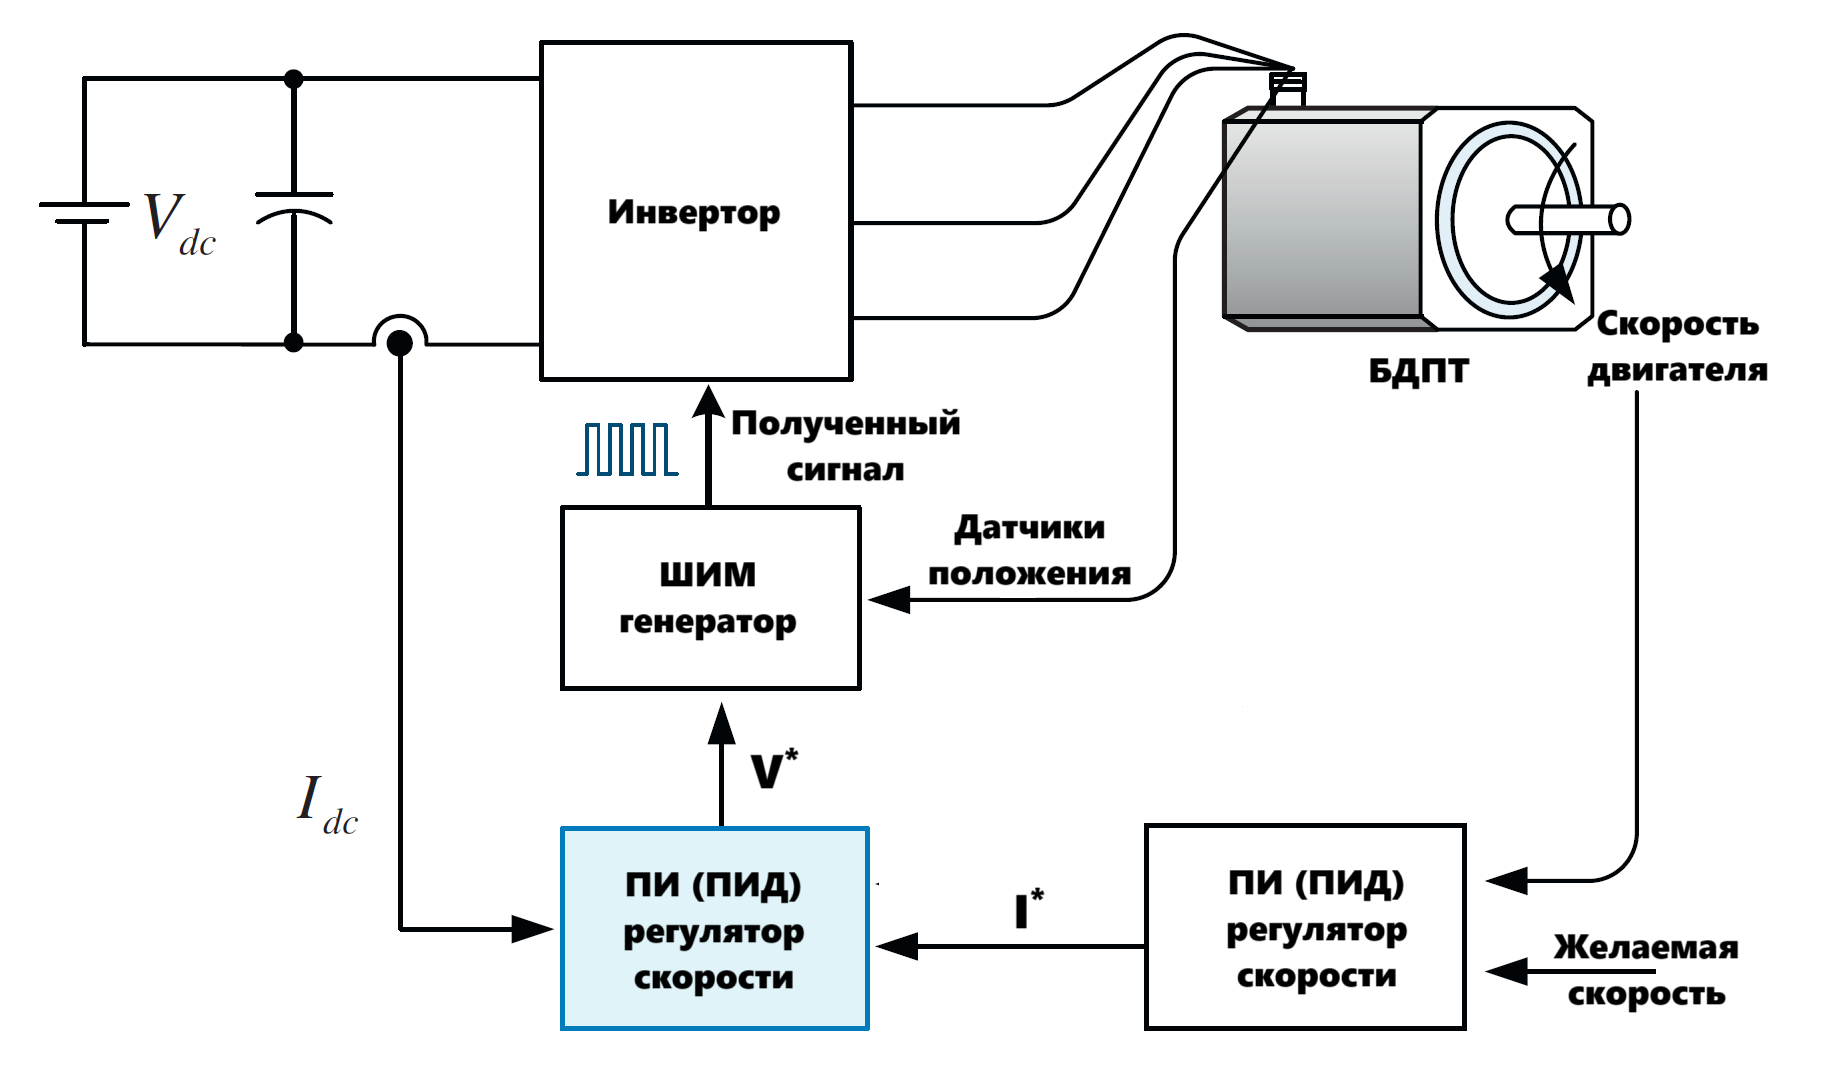
\includegraphics[width=0.7\textwidth]{inc/img/pid2.png}
\caption{Двухконтурная система регулирования скорости \cite{book.kim_motors}}
\label{pic:pid2}
\end{figure}

Для этого подхода необходимо в систему помимо датчиков положения ротора добавить датчик тока.

Использование второго контура позволяет ограничить пульсации тока во время старта и коммутации (смены питаемых обмоток), тем самым ограничив пульсации момента (ведь ток и момент связаны). Однако на практике у нас они всё равно остаются. 

Пульсации момента могут быть вызваны несколькими причинами: особенностями структуры двигателя (несинусоидальный ток и противо-ЭДС из-за питания от постоянного тока и 6-шаговой алгоритмом управления), неэффективной коммутацией во время смены фаз. Особенно сильно они заметны при переменной нагрузки. На Рисунке \ref{pic:commut} приведены графики изменения момента во время коммутации на различных скоростях.

\begin{figure}[!h]
\centering
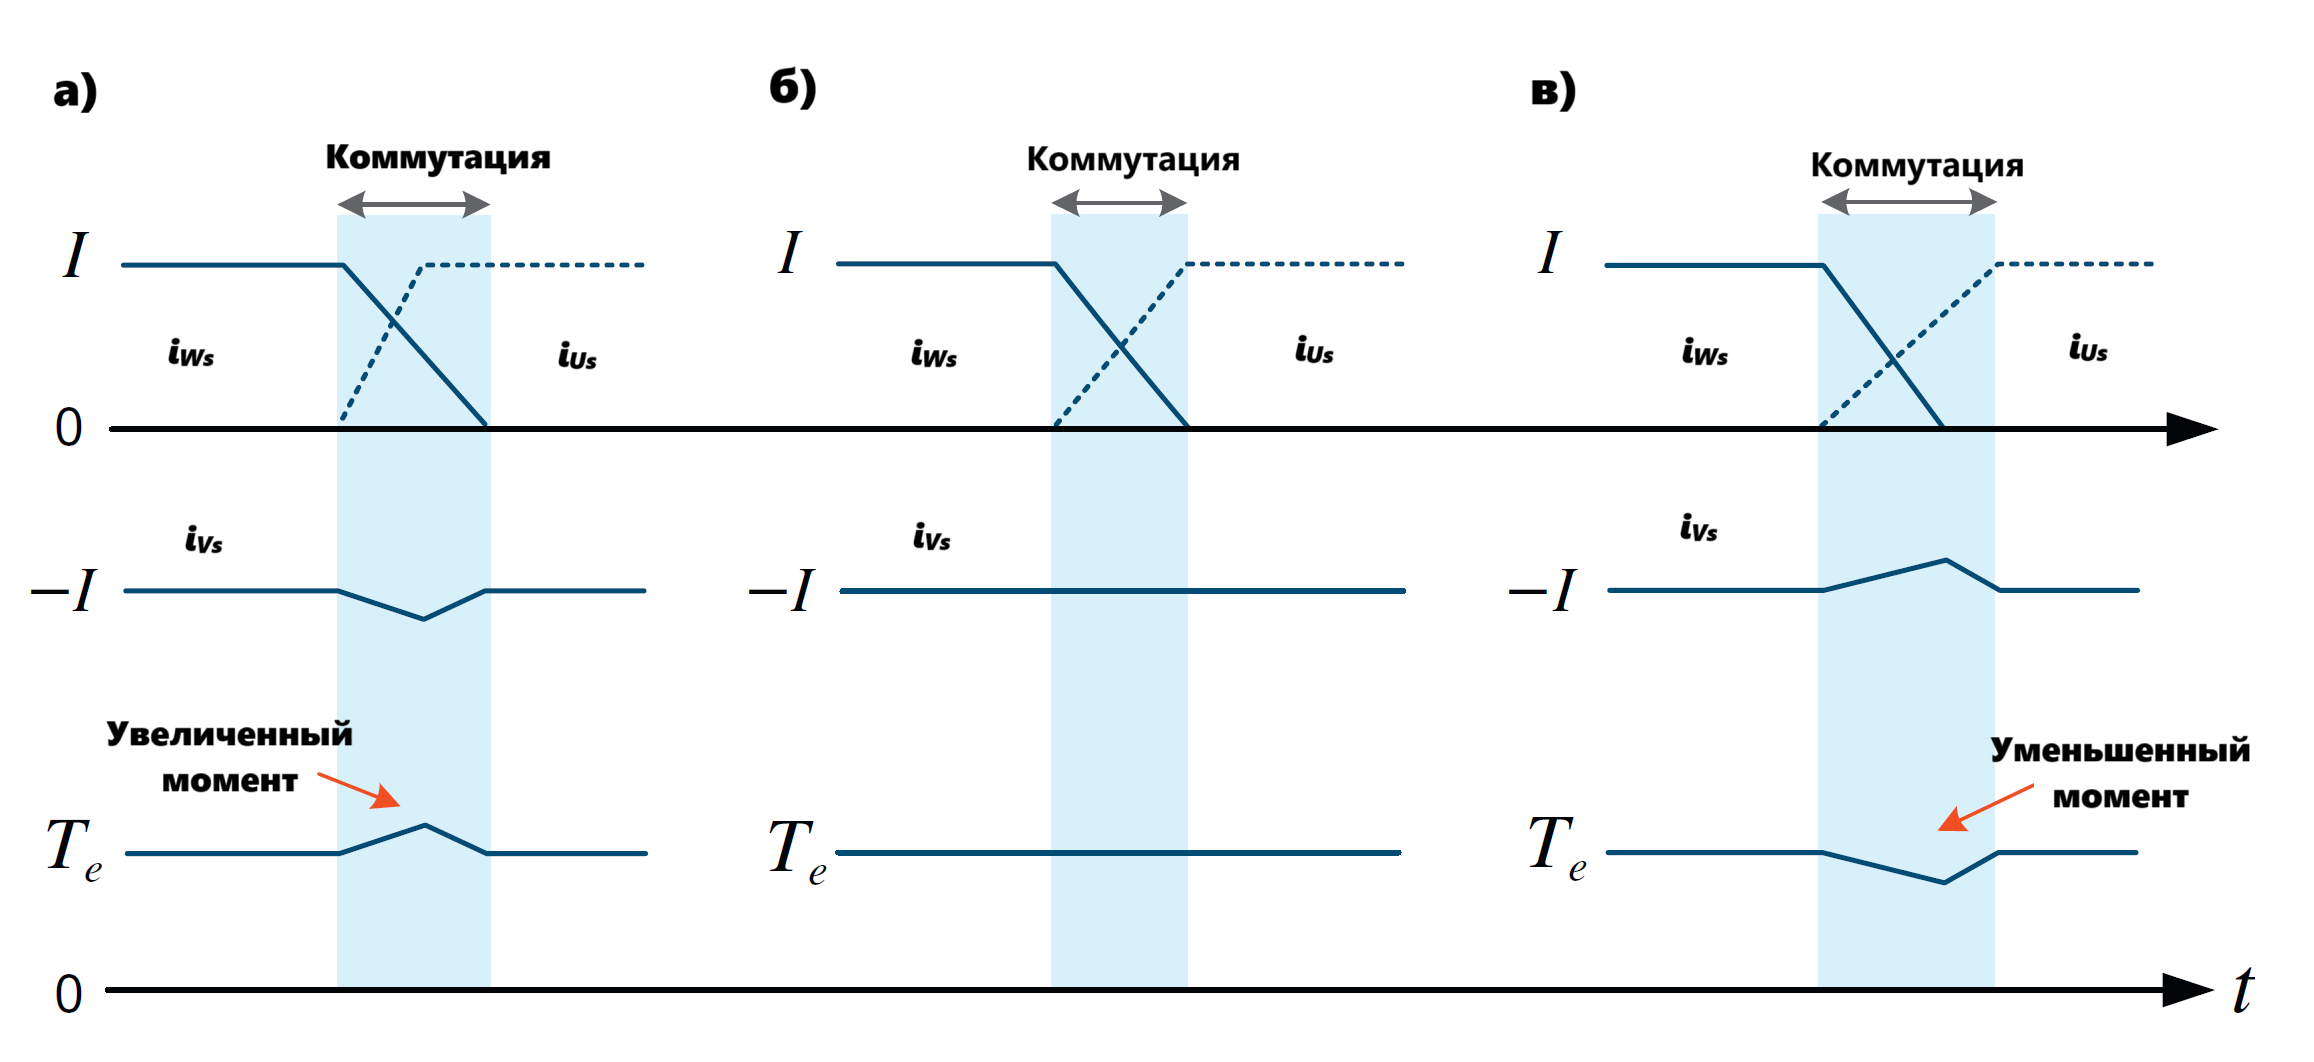
\includegraphics[width=\textwidth]{inc/img/torque_ripple.png}
\caption{Пульсации момента БДПТ на различных скоростях (а --- малые скорости ($V_{dc}>4E$), б --- средние скорости ($V_{dc}=4E$), в --- высокие скорости ($V_{dc}<4E$) ($E$ --- амплитуда противо-ЭДС)) \cite{book.kim_motors}}
\label{pic:commut}
\end{figure}

Для решения этой проблемы применяются более современные алгоритмы, рассмотренные далее.

\section{Векторное управление (FOC)}
\label{sec:foc}

Одной из самых ранних техник для уменьшения пульсаций момента является векторное управление или field orientation control (FOC). Данный алгоритм используется для независимого управления тремя параметрами двигателя (скоростью, потокосцеплением и моментом) и помогает получить форму тока статора, приближенную к синусоидальной (из-за использования синусоидального алгоритма коммутации вместо 6-шагового алгоритма), что позволяет достичь максимальный момент, располагая постоянно магнитные поля ротора и статора перпендикулярно друг другу. Возможная схема реализации этого алгоритма приведена на Рисунке \ref{pic:foc}.

\begin{figure}[!h]
\centering
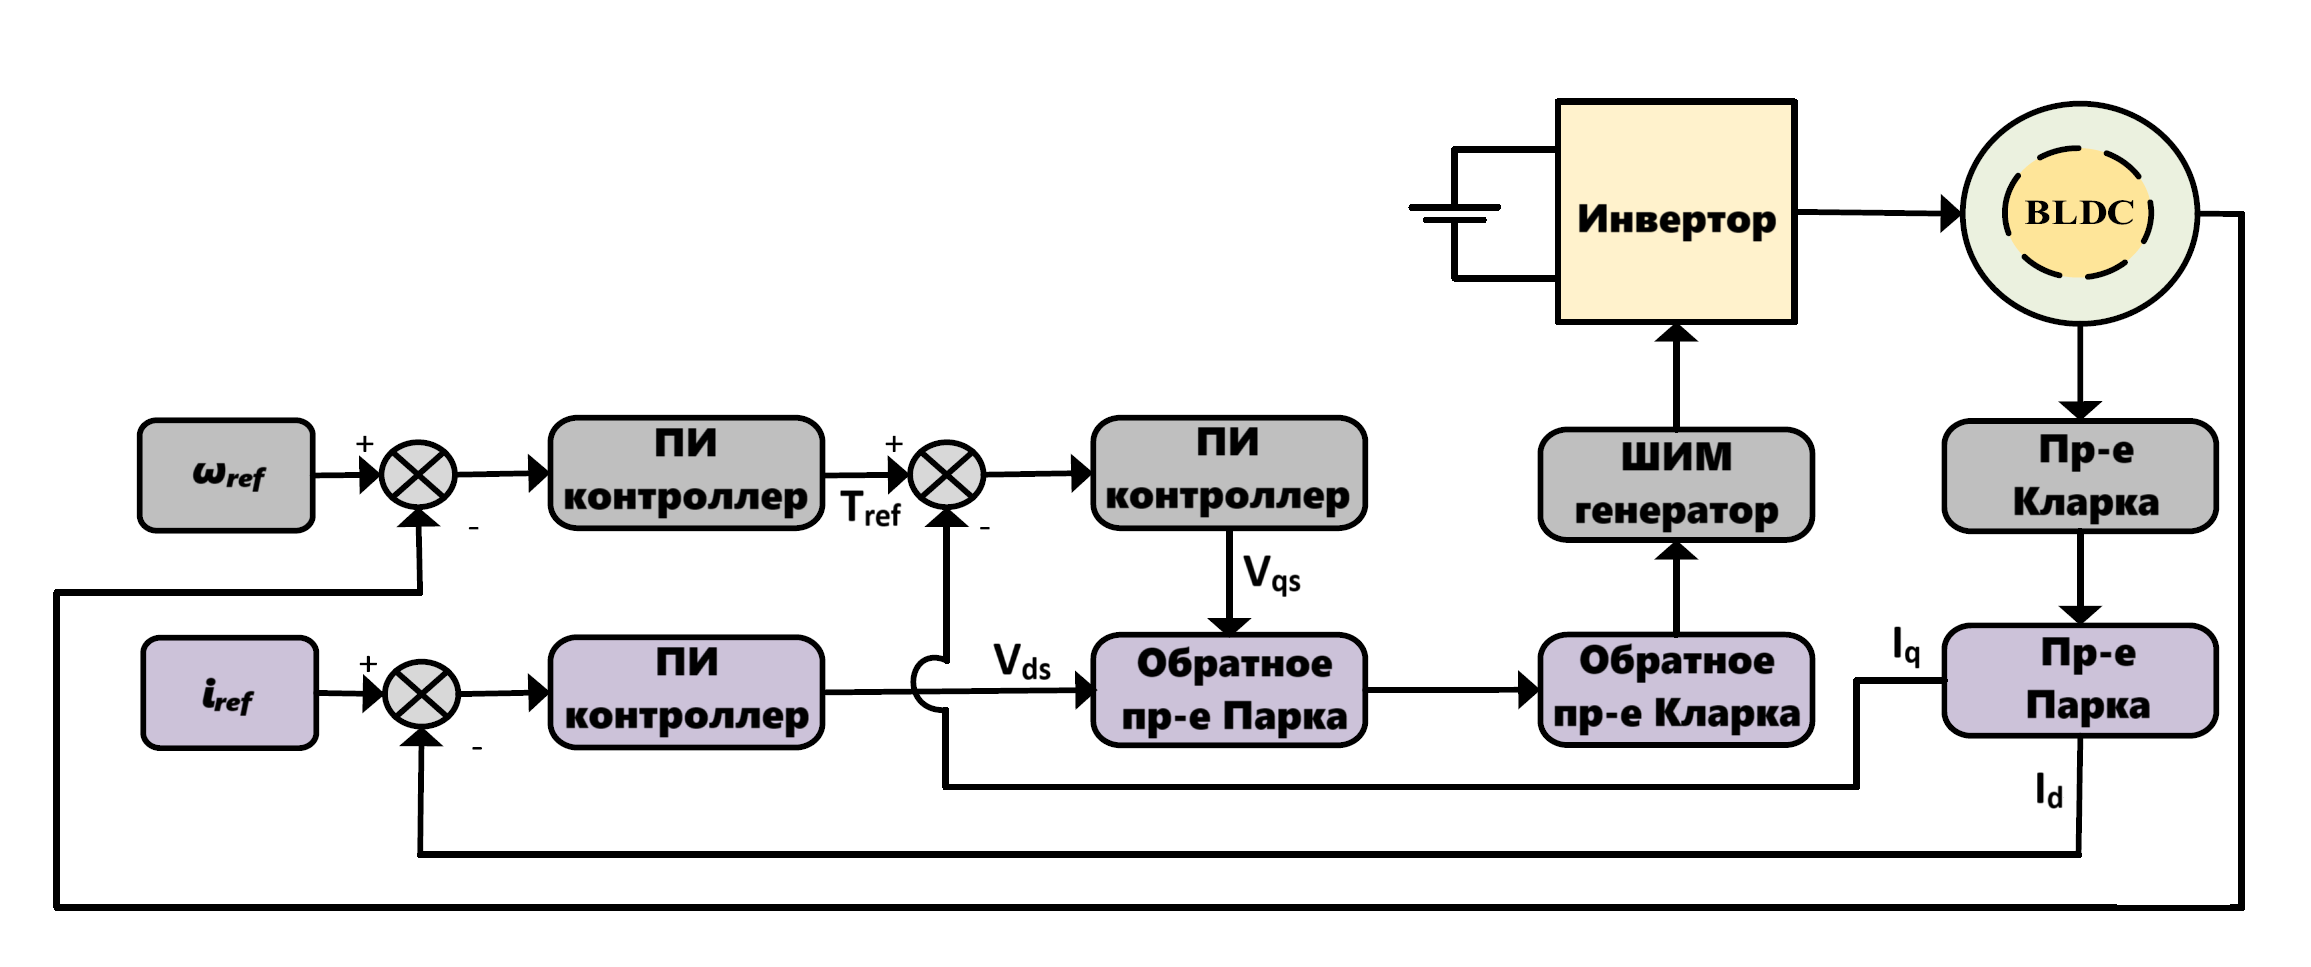
\includegraphics[width=\textwidth]{inc/img/foc.png}
\caption{Система регулирования для векторного управления ($\omega_{ref}$, $i_{ref}$ --- заданные скорость и ток регулирования; $I_d$, $I_q$ --- токи после выполнения преобразования Парка; $V_{ds}$, $V_{qs}$ --- новые векторы напряжения в $d-q$ системе координат) \cite{art:bdlc_adv_control_techs}}
\label{pic:foc}
\end{figure}

Возможный алгоритм функционирования данного типа управления \cite{art:foc_control}:
\begin{enumerate}
	\item определение токов фаз двигателя с использованием соотношения:
	\[
		i_W+i_V+i_U=0
	\]
	\item приведение трёх фазного тока к двухкоординатной системе с использованием преобразования Кларка:
	\begin{align*}
		&i_{\alpha}=i_W \\
		&i_{\beta}=(i_W+2i_V)/\sqrt{3}
	\end{align*}
	\item двухкоординатная система преобразуется для согласования с потокосцеплением ротора (вращаем для совпадения с потоком ротора на основе его угла поворота $\theta$), т. е. выполняется преобразование Парка (или преобразование во вращающуюся систему координат):
	\begin{align*}
		&I_d=i_{\alpha}\cos\theta+i_{\beta}\sin\theta\\
		&I_q=-i_{\alpha}\sin\theta+i_{\beta}\cos\theta
	\end{align*}
	\item использование полученных векторов как входов двух ПИ регуляторов для формирования на выходе векторов напряжений --- $V_{dc}$ и $V_{qs}$. $I_d$ составляющая относится к току или потокосцеплению и в качестве заданного значения используется $0$ для уменьшения пульсаций момента. $I_q$ относится к моменту. 
	\item выполнение обратного преобразования Парка:
	\begin{align*}
		&V_{\alpha}=V_{dc}\cos\theta-V_{qs}\sin\theta \\
		&V_{\beta}=V_{dc}\sin\theta+V_{qs}\cos\theta
	\end{align*}
	\item выполнение обратного преобразования Кларка:
	\begin{align*}
		&V_W=V_{\beta}\\
		&V_V=(-V_{\beta}+\sqrt{3}V_{\alpha})/2\\
		&V_U=(-V_{\beta}-\sqrt{3}V_{\alpha})/2
	\end{align*}
	\item полученные напряжения используются для генерации ШИМ сигнала на основе алгоритма SVPWM (пространственно-векторная широтно-импульсная модуляции) или SPWM (синусоидальная широтно-импульсная модуляция).
\end{enumerate}

Хоть данный метод и позволяет уменьшить пульсации момента, но для его нормального функционирования необходимо наличие датчиков положения ротора. Конечно, можно управлять и бездатчиковым методом, но обычно это выполняется с использованием наблюдателей положения и скорости на основе оценки противо-ЭДС, что требует больше вычислительных мощностей, больше информации о двигателе и является менее надёжным.

\section{Прямое управление моментом (DTC)}

В основе данного метода лежит оценка электромагнитного момента на основе тока и напряжения фаз статора и электрического положения ротора, и его последующее регулирование. Возможная схема реализации этого алгоритма приведена на Рисунке \ref{pic:dtc}.

\begin{figure}[!h]
\centering
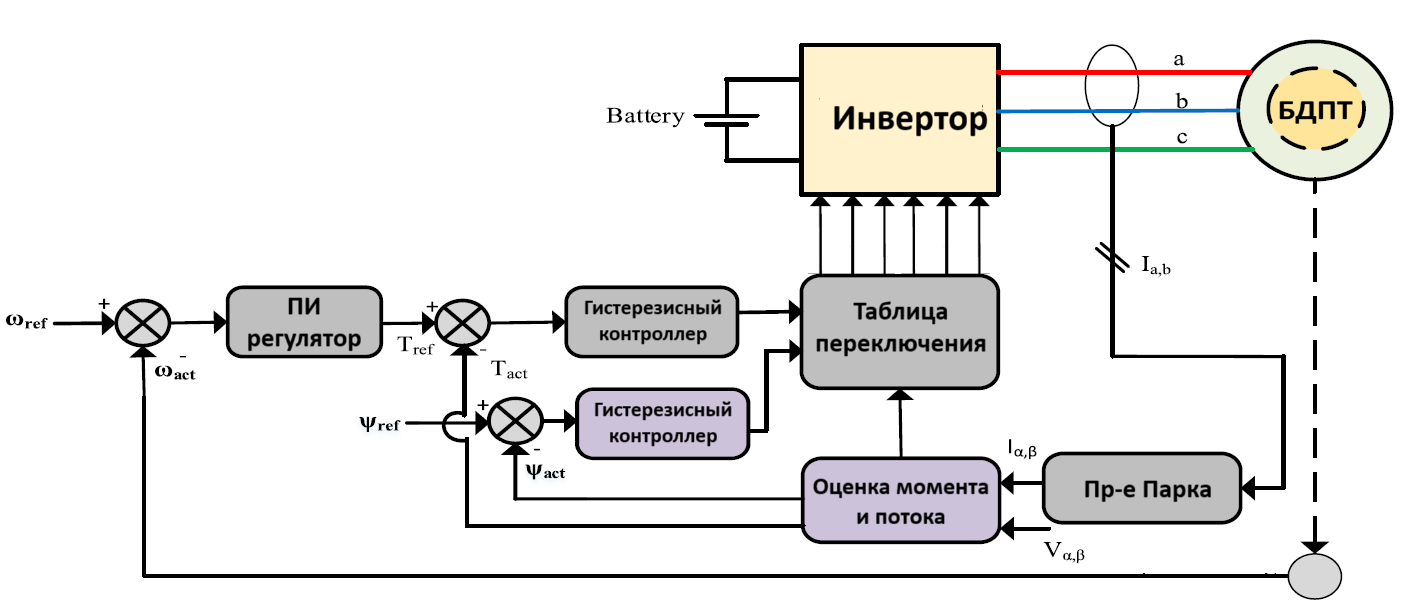
\includegraphics[width=\textwidth]{inc/img/dtc.png}
\caption{Система регулирования для прямого управления моментом ($\omega_{m(ref)}$, $M_{e(ref)}$ --- заданные скорость и момент регулирования; $\omega_{m(act)}$, $\omega_{e(hat)}$ --- текущая скорость и оценка момента; $I_{\alpha\beta}$, $V_{\alpha\beta}$ --- токи и напряжения после выполнения преобразования Кларка) \cite{art:bdlc_adv_control_techs}}
\label{pic:dtc}
\end{figure}

Возможный алгоритм работы следующий:
\begin{enumerate}
	\item выполнить переход к двумерной системе координат для тока и напряжения фаз путём выполнения преобразования Кларка, определить угол положения ротора в электрических градусах;
	\item оценить на основе полученных данных электромагнитный момент двигателя;
	\item получить ошибки по моменту, взяв за желаемое значение выход ПИ регулятора контура скорости;
	\item пропустить ошибки через ПИ или гистерезисные контроллеры (последние представляют в самом простом случае функцию переключения с гистерезисом, которые на выходе имеют $1$ при превышении верхнего порога и $-1$ при выхода за нижний порог);
	\item на основе полученных значений выходов и текущего положения ротора получить новые состояния ключей инвертора согласно специальной таблице коммутации.
\end{enumerate}

Данный метод является менее требовательным в плане вычислительных мощностей, обладает большей робастностью по отношению к параметрам двигателя и обладает лучшими динамическими свойствами по сравнению с векторным управлением. Однако для его нормального функционирования необходима большая частота работы регулятора (большой период дискретизации), особенно при использовании гистерезисных регуляторов, отчего зависят напрямую амплитуды пульсаций момента и скорости. Также он обладает меньшей эффективностью по сравнению с векторным управлением, но при этом его простота позволяет просто реализовать и настроить (нужно лишь найти подходящие параметры ПИ регуляторов и/или выставить пороги гистерезисных регуляторов).